\subsection{FUNCTORIAL PROPERTIES OF K-DIFFERENTIALS}

PROPOSITION 19. Let

\[
\begin{array}{c c c} \mathrm{K} & \xrightarrow {\rho} & \mathrm{K} ^ {\prime} \\ \Big \downarrow_ {\eta} & & \Big \downarrow_ {\eta^ {\prime}} \\ \mathrm{A} & \xrightarrow {u} & \mathrm{A} ^ {\prime} \end{array}
\]

be a commutative diagram of commutative ring homomorphisms, \(\eta\) (resp. \(\eta'\) ) making

A (resp. A') into a K-algebra (resp. K'-algebra). There exists one and only one A-linear mapping \(v: \Omega_{\mathbf{K}}(\mathbf{A}) \to \Omega_{\mathbf{K}'}(\mathbf{A}')\) rendering commutative the diagram

\pandocbounded{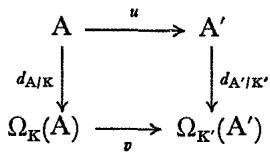
\includegraphics[keepaspectratio]{images/part004_9ff9737d.jpg}}

\(d_{\mathbf{A}^{\prime} / \mathbf{K}^{\prime}}\circ u\) is a K-derivation of A with values in the A-module \(\Omega_{\mathbf{K}^{\prime}}(\mathbf{A}^{\prime})\) ; the existence and uniqueness of \(v\) then follow from Proposition 18 of no. 11.

The mapping v of Proposition 19 will be denoted by \(\Omega(u)\) ; if there is a commutative diagram of commutative ring homomorphisms

\pandocbounded{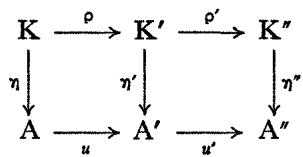
\includegraphics[keepaspectratio]{images/part004_26fbb1e8.jpg}}

it follows immediately from the uniqueness property of Proposition 19 that

\[
\Omega (u ^ {\prime} \circ u) = \Omega (u ^ {\prime}) \circ \Omega (u).
\]

Since \(\Omega_{\mathbf{K}'}(\mathbf{A}')\) is an \(\mathbf{A}'\) -module, from \(\Omega(u)\) we derive canonically an \(\mathbf{A}'\) -linear mapping

\[
\Omega_ {0} (u): \Omega_ {\mathbf {K}} (\mathrm{A}) \otimes_ {\mathrm{A}} \mathrm{A} ^ {\prime} \rightarrow \Omega_ {\mathbf {K} ^ {\prime}} (\mathrm{A} ^ {\prime})\tag{41}
\]

such that \(\Omega(u)\) is the composition of \(\Omega_0(u)\) and the canonical homomorphism \(i_{\mathbf{A}}: \Omega_{\mathbf{K}}(\mathbf{A}) \to \Omega_{\mathbf{K}}(\mathbf{A}) \otimes_{\mathbf{A}} \mathbf{A}'\) . For every \(\mathbf{A}'\) -module \(\mathbf{E}'\) , there is a commutative diagram

\pandocbounded{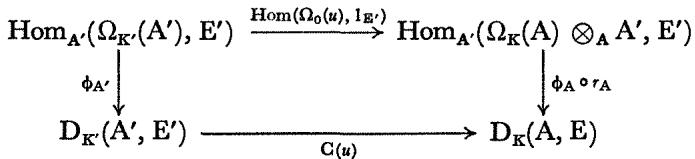
\includegraphics[keepaspectratio]{images/part004_95f64194.jpg}}

where \(\mathbf{C}(u)\) is the mapping \(D \mapsto D \circ u\) (no. 7, Proposition 9) and \(r_{A}\) is the canonical isomorphism

\[
\operatorname{Hom} \left(i _ {\mathrm{A}}, 1 _ {\mathrm{E} ^ {\prime}}\right): \operatorname{Hom} _ {\mathrm{A} ^ {\prime}} \left(\Omega_ {\mathrm{K}} (\mathrm{A}) \otimes_ {\mathrm{A}} \mathrm{A} ^ {\prime}, \mathrm{E} ^ {\prime}\right)\rightarrow \operatorname{Hom} _ {\mathrm{A}} \left(\Omega_ {\mathrm{K}} (\mathrm{A}), \mathrm{E} ^ {\prime}\right);
\]

this follows immediately from Proposition 19 and the definition of the isomorphisms \(\phi_{\mathbf{A}}\) and \(\phi_{\mathbf{A}^{\prime}}\) .

PROPOSITION 20. Suppose that \(\mathbf{A}' = \mathbf{A} \otimes_{\mathbb{K}} \mathbf{K}'\) , with \(\eta': \mathbf{K}' \to \mathbf{A}'\) and \(u: \mathbf{A} \to \mathbf{A}'\) the canonical homomorphisms. Then the \(\mathbf{A}'\) -linear mapping

\[
\Omega_ {0} (u): \Omega_ {\mathbf {K}} (\mathrm{A}) \otimes_ {\mathbf {A}} \mathrm{A} ^ {\prime} \rightarrow \Omega_ {\mathbf {K} ^ {\prime}} (\mathrm{A} ^ {\prime})
\]

is an isomorphism.

By virtue of the fact that in diagram (42) the vertical arrows are bijective, it reduces to proving that, for every A'-module E', the homomorphism C(u):D → D ∘ u in diagram (42) is bijective (II, § 2, no. 1, Theorem 1). Now Hom(u, 1\_E') : Hom\_K'(A ⊗\_K K', E') → Hom\_K(A, E') is an isomorphism (II, § 5, no. 1, Proposition 1) and C(u) is its restriction to D\_K'(A', E') and hence is injective; moreover, if f: A' → E' is a K'-linear mapping such that

\[
f \circ u: \mathrm{A} \rightarrow \mathrm{E} ^ {\prime}
\]

is a K-derivation, it follows immediately from the fact that \(f\) is \(\mathbf{K}'\) -linear and the fact that \(f((x \otimes 1)(y \otimes 1)) = (y \otimes 1)f(x \otimes 1) + (x \otimes 1)f(y \otimes 1)\) for \(x, y\) in A, that \(f\) is a \(\mathbf{K}'\) -derivation, the elements \(x \otimes 1\) for \(x \in A\) forming a generating system of the \(\mathbf{K}'\) -module \(A'\) ; this completes the proof that \(C(u)\) is bijective.

From now on we confine our attention to the case where \(\rho: \mathbf{K} \to \mathbf{K}'\) is the identity mapping of \(\mathbf{K}\) ; every K-algebra homomorphism \(u: \mathbf{A} \to \mathbf{B}\) is therefore mapped to a B-linear mapping

\[
\Omega_ {0} (u): \Omega_ {\mathbf {K}} (\mathrm{A}) \otimes_ {\mathbf {K}} \mathrm{B} \rightarrow \Omega_ {\mathbf {K}} (\mathrm{B}).\tag{43}
\]

On the other hand, we can consider the B-module of A-differentials \(\Omega_{\mathbf{A}}(\mathbf{B})\) since B is an A-algebra by means of u; the canonical derivation \(d_{\mathrm{B/A}}: \mathbf{B} \to \Omega_{\mathbf{A}}(\mathbf{B})\) being a fortiori a K-derivation, it factorizes uniquely into

\[
\mathbf {B} \xrightarrow {d _ {\mathbf {B} / \mathbf {K}}} \Omega_ {\mathbf {K}} (\mathbf {B}) \xrightarrow {\Omega_ {u}} \Omega_ {\mathbf {A}} (\mathbf {B})
\]

where \(\Omega_{u}\) is a B-linear mapping (no. 11, Proposition 18). For every B-module E, there is a commutative diagram

\[
\begin{array}{c} \operatorname{Hom} _ {\mathbf {B}} (\Omega_ {\mathbf {A}} (\mathbf {B}), \mathrm{E}) \xrightarrow {\operatorname{Hom} (\Omega_ {u} , 1 _ {\mathbf {E}})} \operatorname{Hom} _ {\mathbf {B}} (\Omega_ {\mathbf {K}} (\mathbf {B}), \mathrm{E}) \\ \phi_ {\mathbf {A}, \mathbf {B}} \Biggl \downarrow \\ \mathrm{D} _ {\mathbf {A}} (\mathrm{B}, \mathrm{E}) \xrightarrow [ j _ {u} ]{} \mathrm{D} _ {\mathbf {K}} (\mathrm{B}, \mathrm{E}) \end{array}\tag{44}
\]

where \(j_{u}\) is the canonical injection (no. 7); this follows immediately from Proposition 18 of no. 11.

PROPOSITION 21. The sequence of B-linear mappings

\[
\Omega_ {\mathbf {K}} (\mathrm{A}) \otimes_ {\mathbf {A}} \mathrm{B} \xrightarrow {\Omega_ {0} (u)} \Omega_ {\mathbf {K}} (\mathrm{B}) \xrightarrow {\Omega_ {u}} \Omega_ {\mathbf {A}} (\mathrm{B}) \to 0\tag{45}
\]

is exact.

It reduces to verifying that, for every B-module E, the sequence

\[
\begin{array}{c} 0 \to \operatorname{Hom} _ {\mathrm{B}} (\Omega_ {\mathrm{A}} (\mathrm{B}), \mathrm{E}) \xrightarrow {\operatorname{Hom} (\Omega_ {\mathrm{u}} , 1 _ {\mathrm{E}})} \operatorname{Hom} _ {\mathrm{B}} (\Omega_ {\mathrm{K}} (\mathrm{B}), \mathrm{E}) \\ \xrightarrow {\operatorname{Hom} (\Omega_ {0} (u) , 1 _ {\mathrm{E}})} \operatorname{Hom} _ {\mathrm{B}} (\Omega_ {\mathrm{K}} (\mathrm{A}) \otimes_ {\mathrm{A}} \mathrm{B}, \mathrm{E}) \end{array}
\]

is exact (II, §2, no. 1, Theorem 1); but by virtue of the fact that in the commutative diagrams (42) and (44) the vertical arrows are isomorphisms, it suffices to show that the sequence

\[
0 \longrightarrow \mathrm{D} _ {\mathrm{A}} (\mathrm{B}, \mathrm{E}) \xrightarrow {j _ {u}} \mathrm{D} _ {\mathrm{K}} (\mathrm{B}, \mathrm{E}) \xrightarrow {\mathrm{C} (u)} \mathrm{D} _ {\mathrm{K}} (\mathrm{A}, \mathrm{E})
\]

is exact, which is just Proposition 11 of no. 7.

We consider now the case where the K-algebra homomorphism \(u: \mathbf{A} \to \mathbf{B}\) is surjective; if \(\mathfrak{J}\) is its kernel, \(\mathbf{B}\) is then isomorphic to \(\mathbf{A} / \mathfrak{J}\) . We consider the restriction \(d| \mathfrak{J}: \mathfrak{J} \to \Omega_{\mathbf{K}}(\mathbf{A})\) of the canonical derivation \(d = d_{\mathbf{A} / \mathbf{K}}\) and the composite A-linear mapping

\[
d ^ {\prime}: \mathfrak {J} \xrightarrow {d | \mathfrak {J}} \Omega_ {\mathrm{K}} (\mathrm{A}) \xrightarrow {i _ {\mathrm{A}}} \Omega_ {\mathrm{K}} (\mathrm{A}) \otimes_ {\mathrm{A}} \mathrm{B}.
\]

Then \(d^{\prime}(\mathfrak{J}^{2}) = 0\) , since, for \(x, y\) in \(\mathfrak{J}\) ,

\[
d ^ {\prime} (x y) = d (x y) \otimes 1 = (x. d y + y. d x) \otimes 1 = d y \otimes u (x) + d x \otimes u (y) = 0
\]

since \(u(x) = u(y) = 0\) . Hence we derive from \(d'\) , by passing to the quotient, an A-linear mapping

\[
\bar {d} \colon \mathfrak {J} / \mathfrak {J} ^ {2} \rightarrow \Omega_ {\mathrm{K}} (\mathrm{A}) \otimes_ {\mathrm{A}} \mathrm{B}
\]

and as \(\mathfrak{J}\) annihilates the A-module \(\mathfrak{J} / \mathfrak{J}^2\) , \(\bar{d}\) is a B-linear mapping.

PROPOSITION 22. Let \(\mathfrak{J}\) be an ideal of the commutative K-algebra A, B = A/ \(\mathfrak{J}\) and \(u:A\to B\) the canonical homomorphism. The sequence of B-linear mappings

\[
\mathfrak {J} / \mathfrak {J} ^ {2} \xrightarrow {\overline {{d}}} \Omega_ {\mathrm{K}} (\mathrm{A}) \otimes_ {\mathrm{A}} \mathrm{B} \xrightarrow {\Omega_ {0} (u)} \Omega_ {\mathrm{K}} (\mathrm{B}) \to 0\tag{46}
\]

is then exact.

Note that \(\Omega_{\mathbf{K}}(\mathbf{A}) \otimes_{\mathbf{A}} \mathbf{B}\) is identified with \(\Omega_{\mathbf{K}}(\mathbf{A}) / \mathfrak{J} \Omega_{\mathbf{K}}(\mathbf{A})\) and that the image of \(\bar{d}\) is the image of \(d(\mathfrak{J})\) in this quotient module; the quotient of \(\Omega_{\mathbf{K}}(\mathbf{A}) \otimes_{\mathbf{A}} \mathbf{B}\) by \(\operatorname{Im}(\bar{d})\) is therefore identified with the quotient \(\Omega_{\mathbf{K}}(\mathbf{A}) / \mathbf{N}\) , where \(\mathbf{N}\) is the sub-A-module generated by \(\mathfrak{J} \Omega_{\mathbf{K}}(\mathbf{A})\) and \(d(\mathfrak{J})\) . Moreover, the composite mapping

\[
\mathrm{A} \xrightarrow {d _ {\mathrm{A} / \mathrm{K}}} \Omega_ {\mathrm{K}} (\mathrm{A}) \longrightarrow \Omega_ {\mathrm{K}} (\mathrm{A}) / \mathrm{N}
\]

is a K-derivation (no. 7, Proposition 9) and, since it is zero on \(\mathfrak{J}\) by definition of N, it defines, when passing to the quotient, a K-derivation \(D_0:B\to \Omega_{\mathbb{K}}(A) / N\) .

Taking account of the uniqueness of the solution of a universal mapping problem, it reduces to proving that, for every B-module E and every K-derivation D: B → E, there exists a unique B-linear mapping g: \(\Omega_{\mathrm{K}}(\mathrm{A})/\mathrm{N} \rightarrow \mathrm{E}\) such that \(D = g \circ D_{0}\) . But, the composite mapping D ∘ u: A → E is a K-derivation (no. 7, Proposition 9) and hence there exists one and only one A-linear mapping f: \(\Omega_{\mathrm{K}}(\mathrm{A}) \rightarrow \mathrm{E}\) such that \(f \circ d_{A/K} = D \circ u\) . This relation shows already that f is zero on \(d(\mathfrak{J})\) ; as also \(\mathfrak{J} E = \{0\}\) since E is a B-module, f is zero on \(\mathfrak{J} \Omega_{\mathrm{K}}(\mathrm{A})\) ; hence f is zero on N and defines, when passing to the quotient, a B-linear mapping g: \(\Omega_{\mathrm{K}}(\mathrm{A})/\mathrm{N} \rightarrow \mathrm{E}\) such that \(g \circ D_{0} = D\) ; the uniqueness of g follows from the uniqueness of f.

It must not be thought that, even if \(u: \mathbf{A} \to \mathbf{B}\) is an injective homomorphism, \(\Omega_0(u): \Omega_{\mathbf{K}}(\mathbf{A}) \otimes_{\mathbf{A}} \mathbf{B} \to \Omega_{\mathbf{K}}(\mathbf{B})\) is injective (Exercise 5). However we have the following proposition:

PROPOSITION 23. Let A be an integral K-algebra, B its field of fractions and \(u: \mathbf{A} \to \mathbf{B}\) the canonical injection. Then \(\Omega_0(u): \Omega_{\mathbf{K}}(\mathbf{A}) \otimes_{\mathbf{A}} \mathbf{B} \to \Omega_{\mathbf{K}}(\mathbf{B})\) is an isomorphism.

Using the fact that in diagram (42) the vertical arrows are bijective, it reduces to proving that, for every vector space E over B, the mapping \(\mathrm{C}(u):\mathrm{D}_{\mathrm{K}}(\mathrm{B},\mathrm{E})\to\mathrm{D}_{\mathrm{K}}(\mathrm{A},\mathrm{E})\) is bijective. But this follows from the fact that every K-derivation of A into E can be extended uniquely to a K-derivation of B into E (no. 5, Proposition 5).

